\documentclass[aspectratio=169]{beamer}

\usetheme{Madrid}
\useinnertheme{circles}
\usecolortheme{default}

\usepackage[utf8]{inputenc}
\usepackage[T5]{fontenc}
\usepackage[vietnamese]{babel}
\usepackage{amsmath}
\usepackage{amssymb}
\usepackage{booktabs}
\usepackage{tikz}
\usetikzlibrary{arrows.meta, positioning}

\hypersetup{
  pdftitle={He thong kiem soat ra vao thong minh - AIoT},
  pdfauthor={Nhom: Quang, Nhan, Van, Phu},
  pdfsubject={Smart Access Control with Camera, RFID and Web Alerts},
}

\title[Chi tiết các thiết bị]{Hệ thống kiểm soát ra vào thông minh}
\subtitle{Camera $\cdot$ RFID/NFC $\cdot$ Cảnh báo web}
\subtitle{Danh sách thiết bị và chi tiết luồng hoạt động của thiết bị}
\author[Nhóm thực hiện]{Lưu Huy Minh Quang -- 23127016 \and Hoàng Nhân -- 23127094 \and Trần Cao Vân -- 23127141 \and Nguyễn Trần Thiên Phú -- 23127246}
\institute[HCMUS]{Khoa Công nghệ Thông tin\\Đại học Khoa học Tự nhiên, ĐHQG TP.HCM\\[0.3em]\textit{Môn: Nhập môn lập trình điều khiển thiết bị thông minh}}
\date{Tháng 6, 2026}

\AtBeginSection[]{
  \begin{frame}[plain]
    \vfill
    \centering
      {\Large Phần \insertsectionnumber}\par\vspace{0.6em}
      {\LARGE\bfseries \insertsectionhead}\par
    \vfill
  \end{frame}
}

\begin{document}

%------- TITLE -------
\begin{frame}
  \begin{center}
    \vspace{0.4em}
    {\usebeamerfont{title}\Large\bfseries\inserttitle\par}
    \vspace{0.3em}
    {\usebeamerfont{subtitle}\insertsubtitle\par}

    \vspace{1.2em}
    {\large\bfseries Nhóm thực hiện}\\[0.6em]
    \begin{tabular}{ll}
      Lưu Huy Minh Quang & 23127016 \\
      Hoàng Nhân & 23127094 \\
      Trần Cao Vân & 23127141 \\
      Nguyễn Trần Thiên Phú & 23127246 \\
    \end{tabular}\\[0.8em]
    \textit{Khoa CNTT -- ĐH Khoa học Tự nhiên, ĐHQG TP.HCM}\\
    \textit{Môn: Nhập môn lập trình điều khiển thiết bị thông minh}

    \vspace{0.8em}
    {\large \insertdate}
  \end{center}
\end{frame}

%------- MỤC LỤC -------
\begin{frame}{Nội dung trình bày}
  \vspace{0.4em}
  \begin{enumerate}
    \item Tóm tắt project
    \item Danh sách thiết bị
    \item Luồng hoạt động của các thiết bị
  \end{enumerate}
\end{frame}

%============================
\section{Giới thiệu project}
%============================

\begin{frame}{Tóm tắt project}
  \textbf{Sản phẩm:} \textbf{hệ thống cổng kiểm soát ra vào thông minh}. Hệ thống kết hợp \textbf{camera}, \textbf{RFID/NFC}, \textbf{servo} và \textbf{web dashboard} để nhận diện người, xác thực mở cửa và gửi cảnh báo khi có xâm nhập.

  \vspace{0.8em}
  3 Mục tiêu thực hiện:
  \begin{enumerate}
    \item Hệ thống dùng camera để phát hiện và nhận diện tối đa \textbf{20 người dùng đã đăng ký} trong phạm vi \textbf{$0.5$ m}, với \textbf{độ chính xác định danh trên $95\%$}, \textbf{tỷ lệ nhận nhầm dưới $2\%$} và thời gian phản hồi \textbf{dưới $1.5$ giây}.
    \item Hệ thống giám sát dựa trên \textbf{cảm biến siêu âm} để phát hiện khoảng cách bất thường tại cổng và dùng \textbf{camera} để chụp \textbf{Snapshot} đẩy lên \textbf{Web AI} xử lý trong vòng \textbf{$2$ giây}. Khi phát hiện hành vi trèo hoặc nhảy qua cổng, hệ thống báo động tại chỗ và gửi cảnh báo lên web để người quản lý xử lý kịp thời.
    \item Hệ thống dùng RFID/NFC để xác thực người dùng hợp lệ và mở cửa tự động \textbf{dưới $2$ giây}, đồng thời đạt \textbf{độ chính xác xác thực tối thiểu $98\%$} trong điều kiện vận hành bình thường.
  \end{enumerate}
\end{frame}

%============================
\section{Danh sách thiết bị}
%============================

\begin{frame}{Danh mục linh kiện dự kiến}
  \scriptsize
  \renewcommand{\arraystretch}{1.2}
  \begin{tabular}{p{0.35cm}p{2.45cm}p{5.9cm}p{0.75cm}p{1.35cm}}
    \toprule
    \textbf{STT} & \textbf{Linh kiện} & \textbf{Chi tiết kỹ thuật} & \textbf{SL} & \textbf{Giá (VNĐ)} \\
    \midrule
    1 & ESP32 CP2102 38P Type-C & Bộ điều khiển trung tâm, giao tiếp USB Type-C & 1 & 123.000 \\
    2 & Cảm biến siêu âm (HC-SR04) & Phát hiện khoảng cách bất thường tại cổng & 1 & 25.000 \\
    3 & Module đọc thẻ RFID RC522 & Đọc UID thẻ RFID/NFC để xác thực người dùng & 1 & 21.000 \\
    4 & Micro Servo SG90 & Điều khiển đóng/mở cơ cấu cổng mô phỏng & 2 & 60.000 \\
    5 & ESP32-CAM AI Thinker & Thu hình Snapshot hỗ trợ nhận diện và xử lý AI & 1 & 200.000 \\
    6 & LED & Hiển thị trạng thái hợp lệ/cảnh báo & 2 & 1.600 \\
    7 & Buzzer & Phát cảnh báo âm thanh tại chỗ & 1 & 3.000 \\
    8 & Điện trở 220 $\Omega$ & Phụ kiện mạch cho LED và tín hiệu điều khiển & 5 & 200 \\
    \midrule
    \multicolumn{4}{r}{\textbf{Tổng cộng:}} & \textbf{434.600} \\
    \bottomrule
  \end{tabular}
\end{frame}


%============================
\section{Chi tiết thiết bị}
%============================
\begin{frame}{1. Mạch điều khiển}
  Hệ thống gồm 2 mạch điều khiển: 
  \begin{enumerate}
    \item ESP32 38 I/O Pin Type C dùng để điều khiển các thiết bị ngoại vi (Cảm biến hồng ngoại, RFID, servo,...), phục vụ mục đích mở cổng và các Mục đích 2 và 3, có khả năng tạo wifi hotspot và kết nối bluetooth, đảm bảo nguồn điện đủ cho các thiết bị kết nối.
    \item ESP32-CAM AI Thinker phục vụ việc áp dụng Thị giác máy tính nhằm nhận diện người dùng đã đăng ký để mở cổng. Bên cạnh đó cũng chụp lại khoảng khắc có người trèo qua cổng vi phạm. ESP32-CAM sẽ không kết nối với bất kì thiết bị nào khác, chỉ đảm nhận việc kết nối wifi, thực hiện nhận diện, gửi dữ liệu qua ESP32 38P.
  \end{enumerate}

  2 mạch này sẽ hoạt động cùng nhau và tương tác với nhau thông qua wifi. Mô hình được nạp thẳng vào ESP32-CAM và chạy ngay trên mạch, từ đó gửi dữ liệu cho ESP32 38P để thực hiện các chức năng của cổng


\end{frame}

\begin{frame}{1. Mạch điều khiển}

\begin{columns}
    \column{0.5\textwidth}
    \centering
    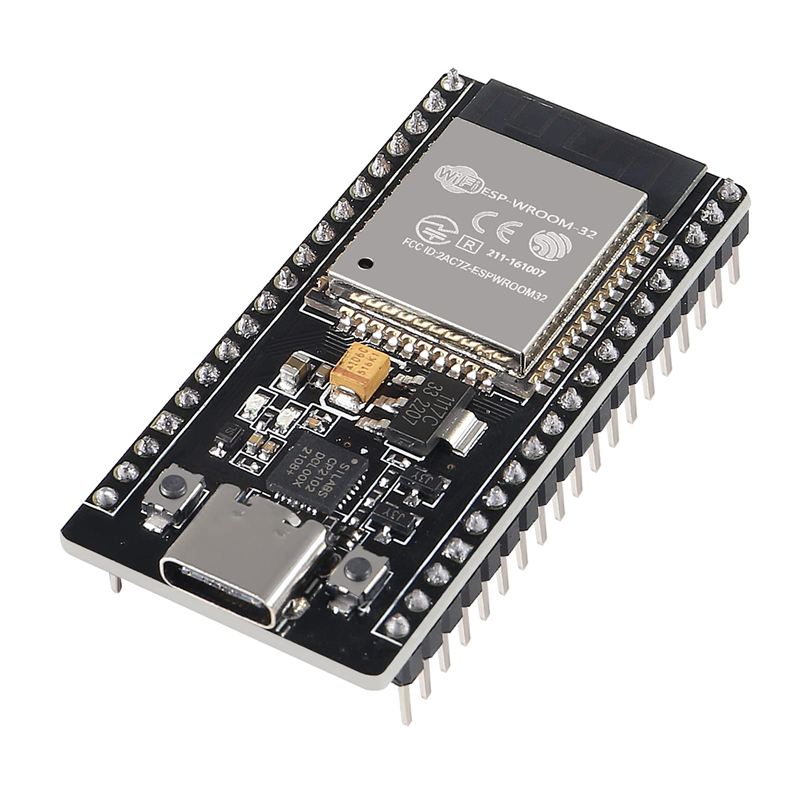
\includegraphics[width=0.6\linewidth]{figures/ESP32 38P.png}
    
    \small Hình 1: ESP32 38P

    \column{0.5\textwidth}
    \centering
    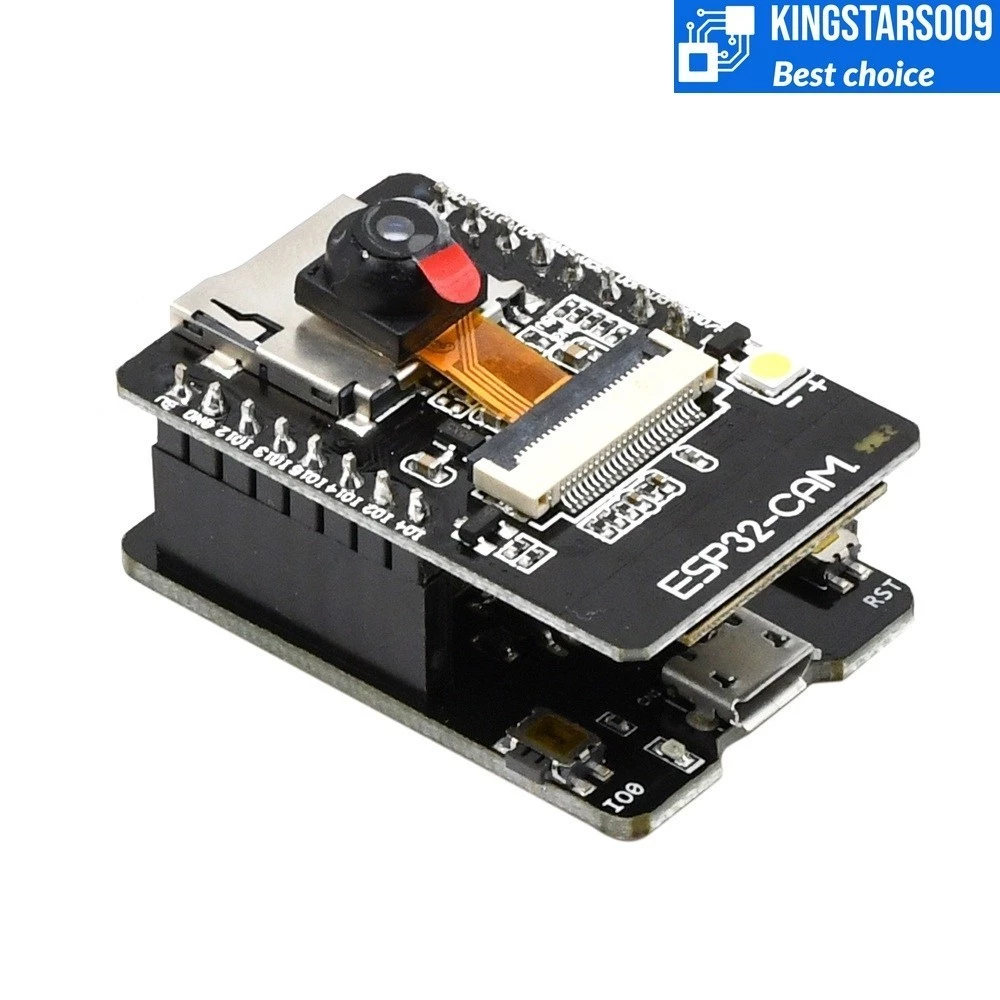
\includegraphics[width=0.6\linewidth]{figures/ESP32 Cam.png}
    
    \small Hình 2: ESP32 CAM
\end{columns}

\end{frame}

\begin{frame}{2. Thiết bị điều khiển cổng}
  Các thiết bị chính điều khiển cổng bao gồm: 
  \begin{enumerate}
    \item HC-SR04 Cảm biến siêu âm: xác nhận xem có người trèo qua cổng không khi cổng đang đóng, phục vụ cho mục đích 2.
    \item RC522 RFID - Cảm biến thẻ từ: Có khả năng đọc và ghi thẻ NFC, hoạt động như cách thứ hai để mở cổng, phục vụ cho mục đích 3
    \item Servo RC SG90 gồm 2 cái để mở 2 bên cổng chịu trách nhiệm chính và là thành phần quan trọng.
  \end{enumerate}

  Các thiết bị hỗ trợ điều khiển cổng được kết nối trực tiếp với ESP32 38P để thực hiện chức năng của mình.


\end{frame}

\begin{frame}{2. Thiết bị điều khiển cổng}

\begin{columns}
    \column{0.5\textwidth}
    \centering
    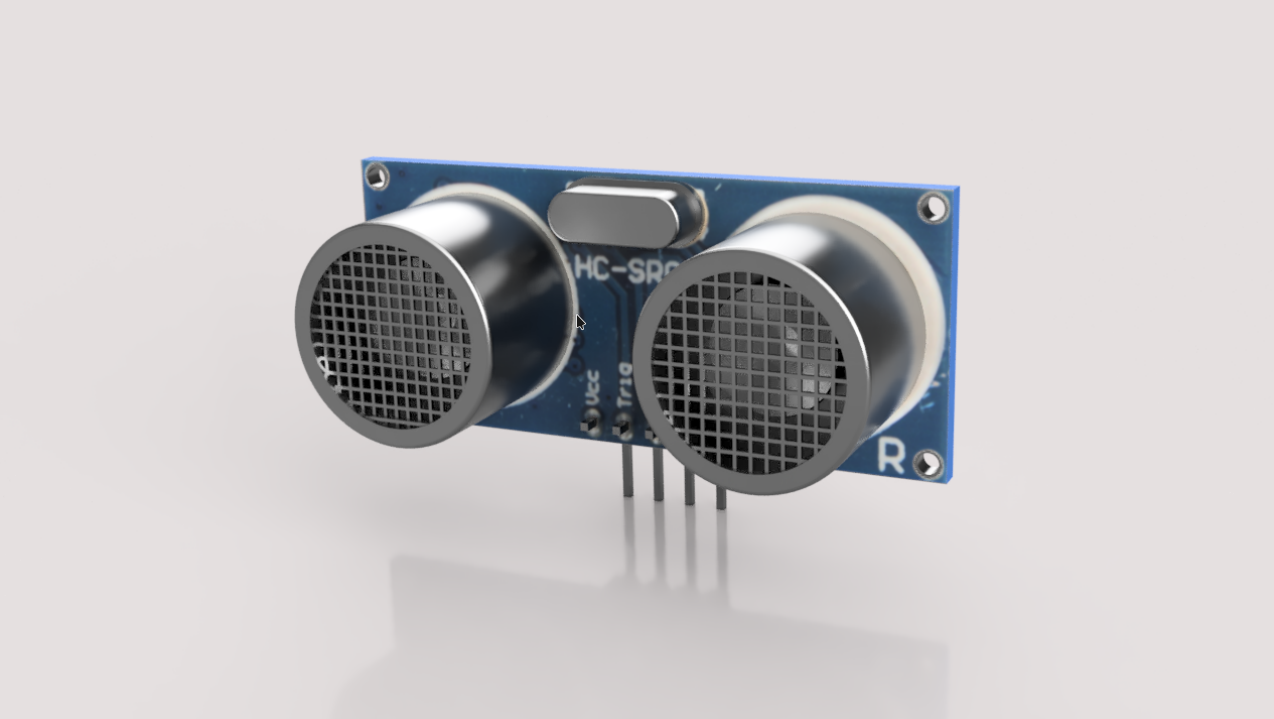
\includegraphics[width=0.4\textwidth]{figures/HCSR04.png}
    
    \small Hình 3: HCSR04

    \column{0.5\textwidth}
    \centering
    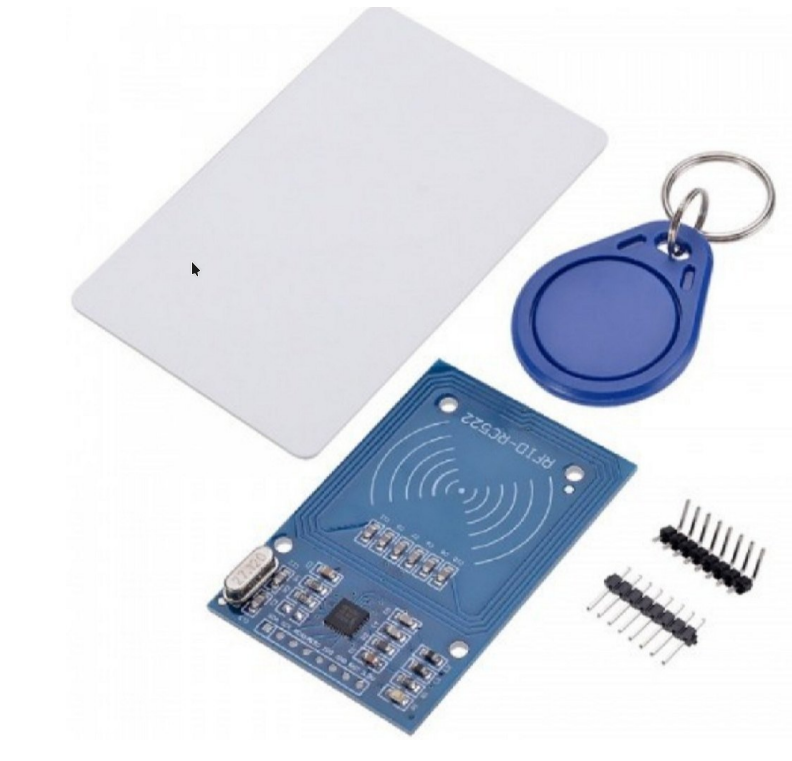
\includegraphics[width=0.4\textwidth]{figures/RC522 RFID.png}
    
    \small Hình 4: RC522 RFID
\end{columns}

\begin{figure}[htbp]
    \centering
    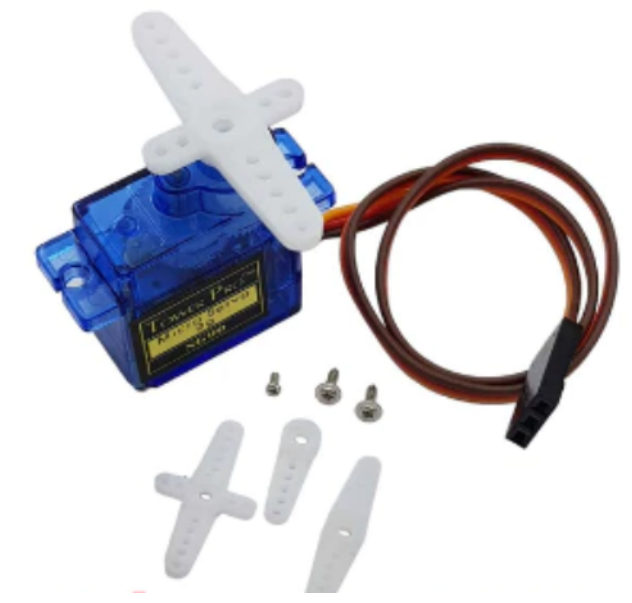
\includegraphics[width=0.2\textwidth]{figures/RC SG90.png}
    \small Hình 5: RC SG90
\end{figure}

\end{frame}

\begin{frame}{3. Thiết bị thông báo}
  Các thiết bị hỗ trợ thông báo khi cổng được mở hoặc có người vi phạm
  \begin{enumerate}
    \item LED 3.3V với 2 màu đỏ và xanh tượng trưng cho cổng được mở và cổng đóng.
    \item Buzzer 5V để phát âm thanh thông báo khi cổng được mở hoặc có người vi phạm. 
    \item Điện trở 220 Ohm để hạn chế dòng điện đi qua LED và Buzzer, đảm bảo thiết bị chạy an toàn và không bị quá tải
  \end{enumerate}

\end{frame}

\begin{frame}{3. Thiết bị thông báo}

\begin{columns}
    \column{0.5\textwidth}
    \centering
    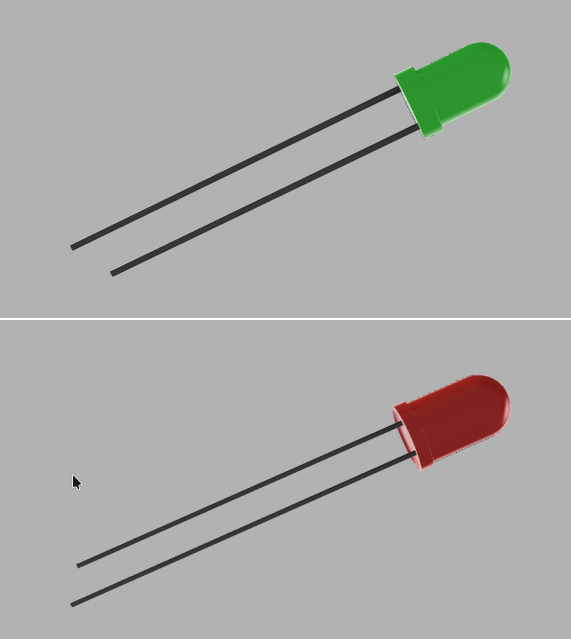
\includegraphics[width=0.3\textwidth]{figures/Led.png}
    
    \small Hình 6: Led đỏ và Led xanh 

    \column{0.5\textwidth}
    \centering
    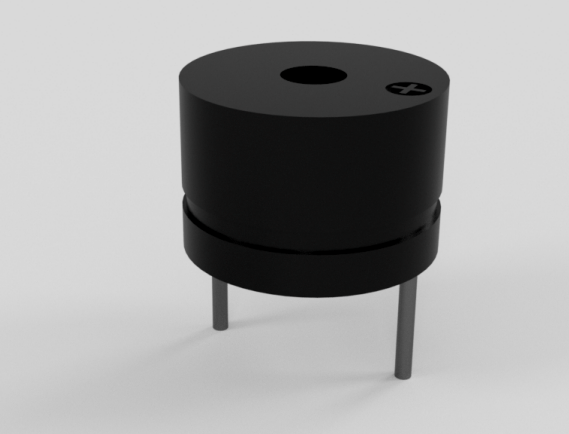
\includegraphics[width=0.4\textwidth]{figures/Buzzer.png}
    
    \small Hình 7: Buzzer 5V
\end{columns}

\begin{figure}[htbp]
    \centering
    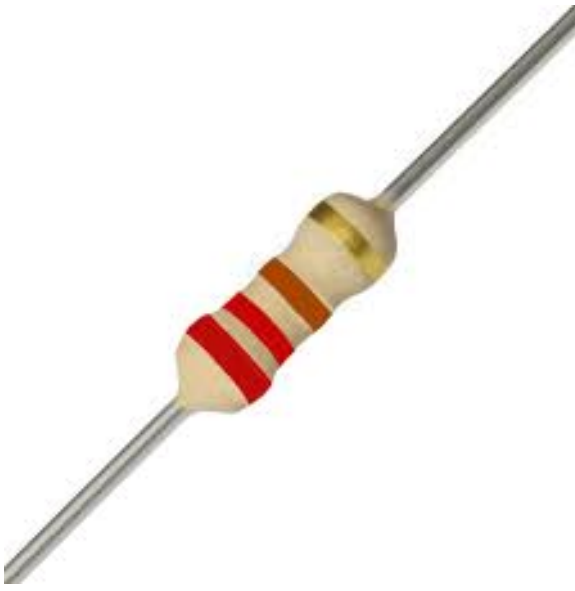
\includegraphics[width=0.15\textwidth]{figures/Dientro.png}
    \small Hình 8: Điện trở 220 Ohm
\end{figure}

\end{frame}

\section{Luồng hoạt động của các thiết bị}

\begin{frame}{1. Luồng hoạt động bằng Camera - Mục đích 1}
\begin{figure}[htbp]
    \centering
    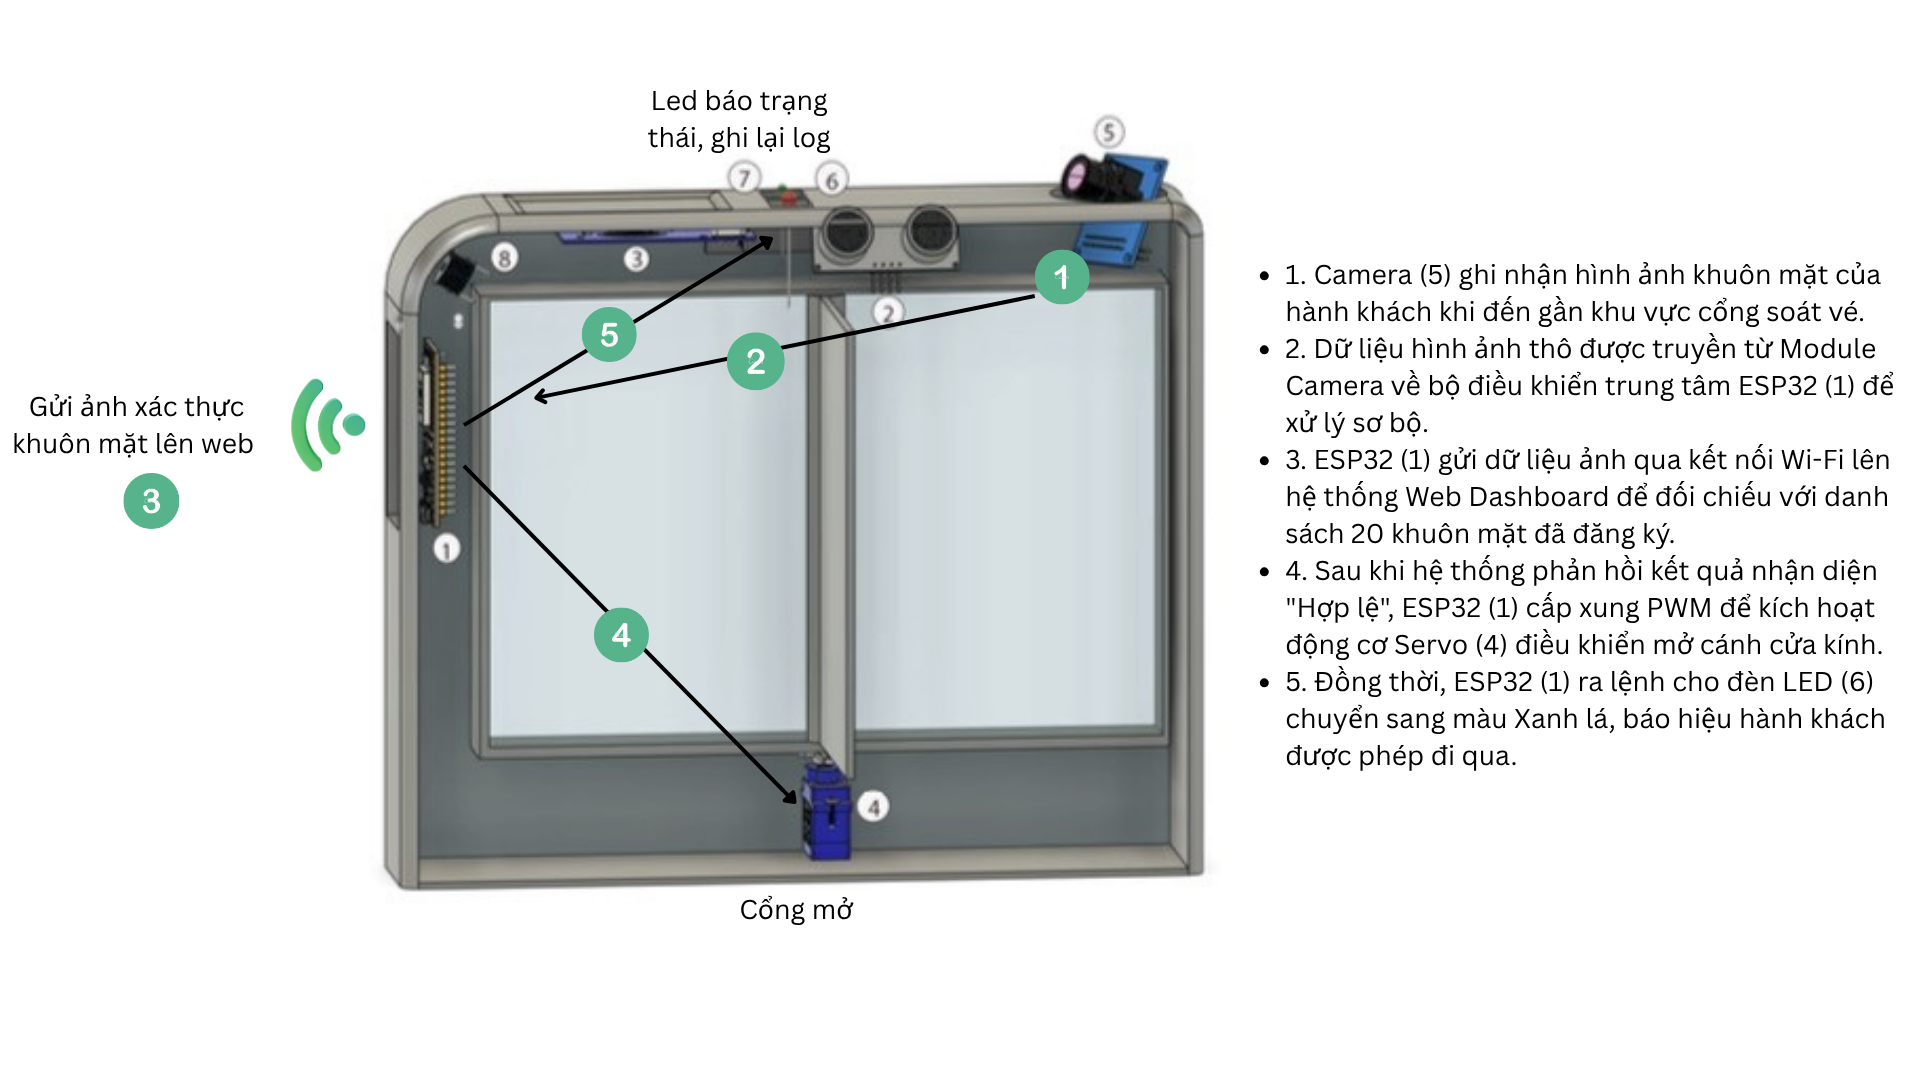
\includegraphics[width=1\textwidth]{figures/Luồng CAM.png}
\end{figure}

  
\end{frame}


\begin{frame}{2. Luồng bắt vi phạm khi xảy ra - Mục đích 2}
\begin{figure}[htbp]
    \centering
    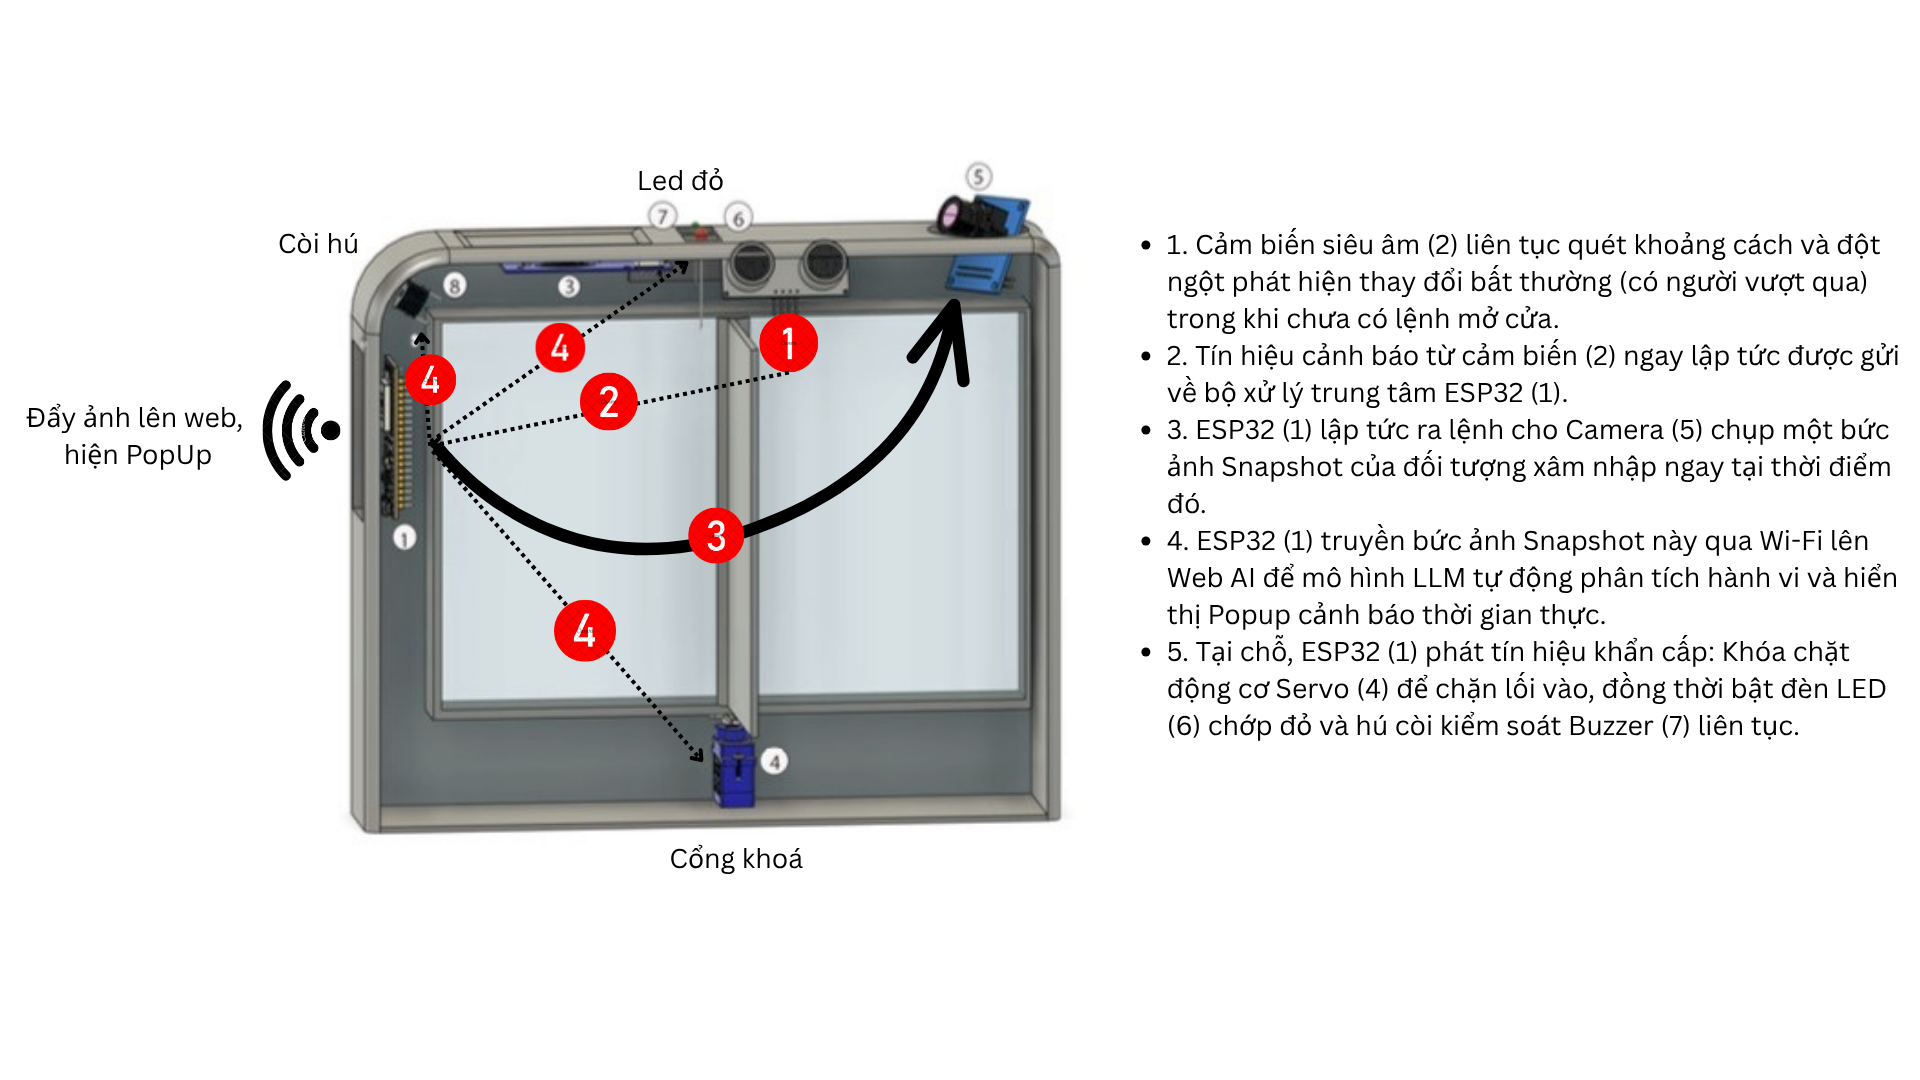
\includegraphics[width=1\textwidth]{figures/Luồng vi phạm.png}
\end{figure}

\end{frame}

\begin{frame}{3. Backup sử dụng RFID để mở cổng - Mục đích 3}
\begin{figure}[htbp]
    \centering
    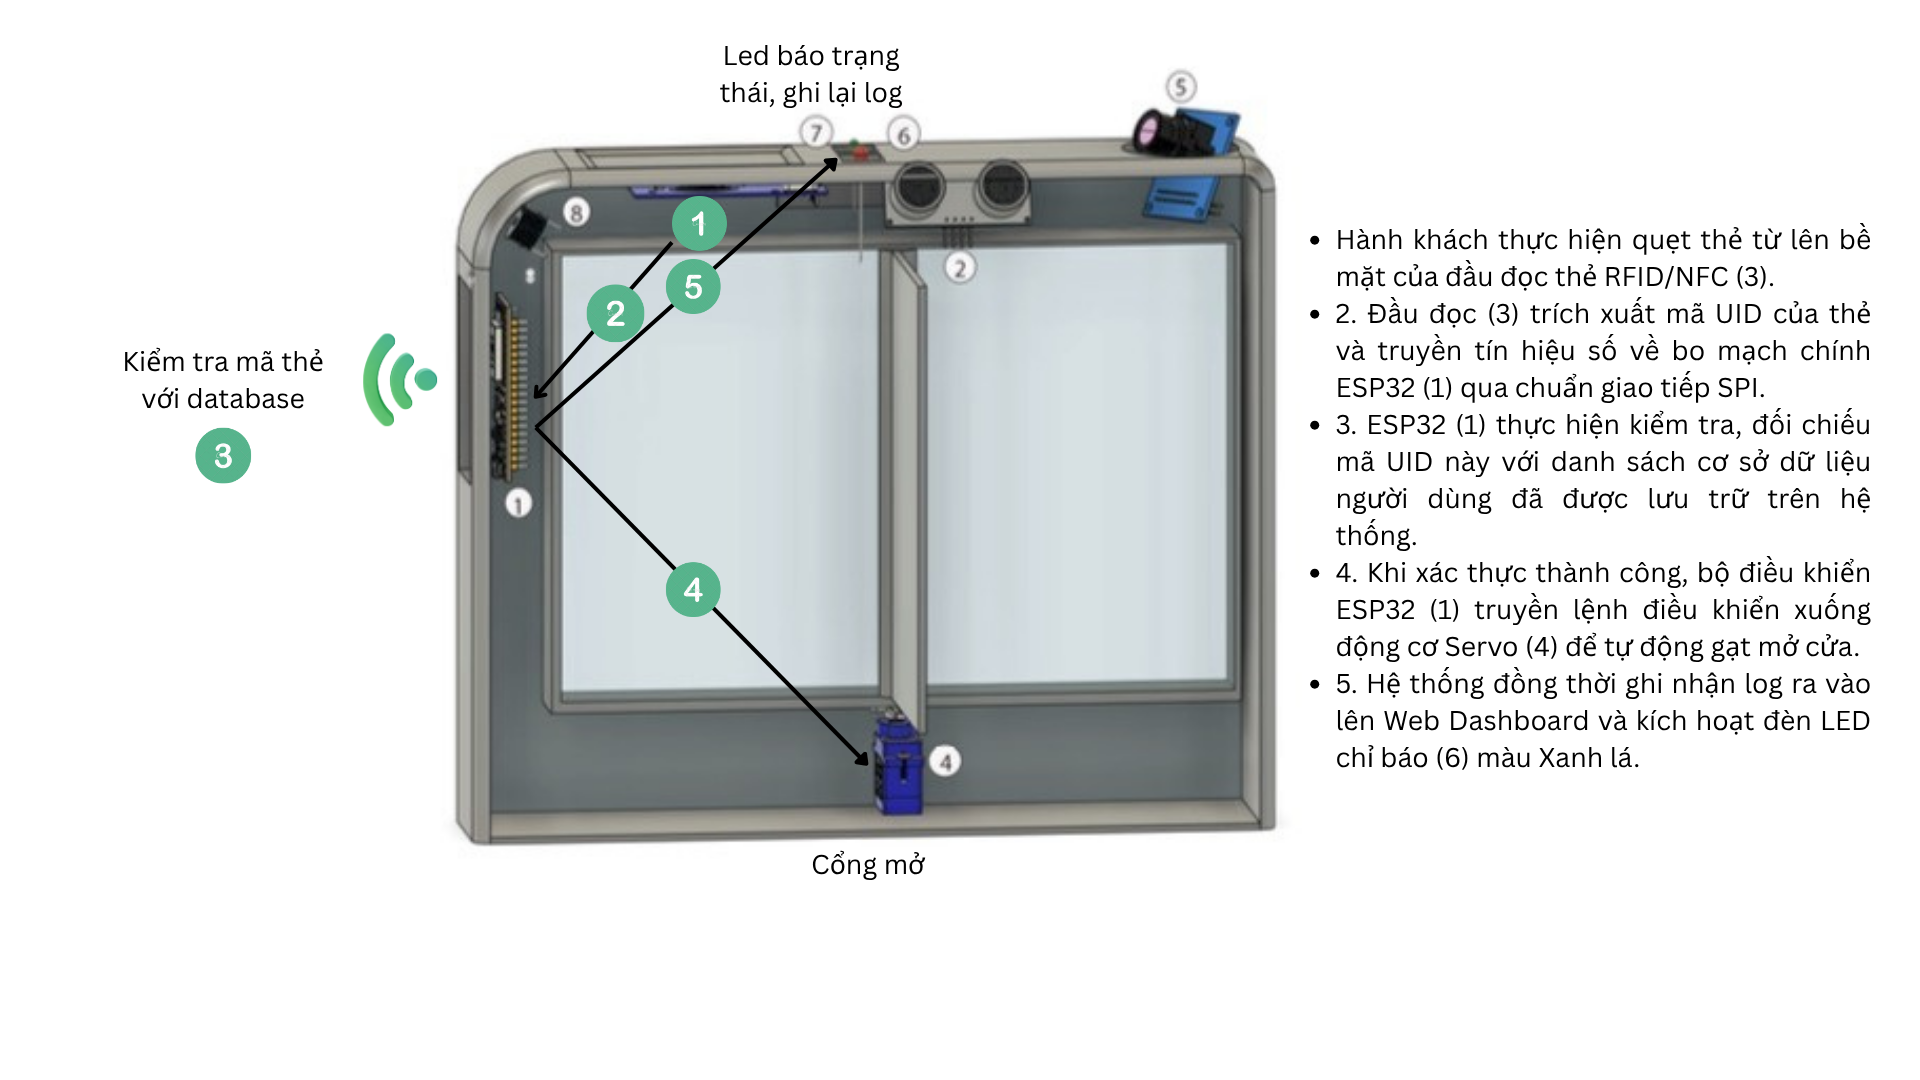
\includegraphics[width=1\textwidth]{figures/Luồng RFIDNFC.png}
\end{figure}

\end{frame}

%------- CLOSING -------
\begin{frame}[plain]
  \begin{center}
    \vspace{2.5cm}
    {\Huge \textbf{Cảm ơn!}}\\[0.8em]
    {\Large Câu hỏi \& Thảo luận}
  \end{center}
\end{frame}

\end{document}
